\documentclass{beamer}
\usetheme{Boadilla}

\usepackage[italian, english]{babel}
\usepackage[utf8]{inputenc}
\usepackage{graphicx}
\usepackage{amsmath}
\usepackage{tikz}
\usetikzlibrary{positioning}

\title{Verifica del Software}
\subtitle{Project 17 (Interpreter, Call-by-name version)}
\author{Nicola Carlesso}
\institute{UniPd - Informatica}
\date{\today}

\begin{document}
	\begin{frame}
		\titlepage
	\end{frame}

\section{Haskell}
\begin{frame}{Haskell}
	\begin{figure}
		
\includegraphics[scale=0.3]{img/haskell-logo}
	\end{figure}
	\begin{itemize}
		\item Pure Functional Language
		\item Lazy Evaluation
		\item Pattern Matching
		\item Tail Recursion
	\end{itemize}
\end{frame}

\section{Parser}
\begin{frame}{The REC language grammar}
	\begin{itemize}
		\item The grammar of REC language:\\
		t ::= n $|$ \text{var} $| t_1 + t_2 | t_1 - t_2 | t_1 * t_2 |$
		if $t_0$ then $t_1$ else $t_2 |$ $f_i(t_1, \dots, t_{ai})$
		\item The grammar of REC language with respect to the precedence of operations:
		\begin{align*}
		expr &::= term + expr | term - minus | term\\
		minus &::= term - minus | term \hspace{0.5cm} \textcolor{red}{Es. (5-2)-1 \neq 5-(2-1)}\\
		term &::= factor * term | factor\\
		factor &::= \text{n } | \text{ var } | t_1 + t_2 | t_1 - t_2 | t_1 * t_2 |
		\text{if } t_0 \text{then } t_1 \text{else } t_2 | f_i(t_1, \dots, t_{ai})
		\end{align*}
		Further more:
		\begin{align*}
		func &::= var(varn)\\
		n &::= \underline{undef} | 0 | 1 | 2 | \dotsc\\
		varn &::= var , varn | var\\
		var &::= \text{``any character''} varch\\
		varch &::= \text{``any character'' } | \text{ ``any digit'' } | \text{ \_ } | varch | \epsilon
		\end{align*}
	\end{itemize}
\end{frame}

\begin{frame}
	\begin{itemize}
		\item The grammar of the input:\\
		\begin{columns}
			\column{0.5\textwidth}
			\begin{align*}
			prog &::= funcn; expr; decn;\\
			funcn &::= func, funcn | func\\
			decn &::= dec, decn | dec\\
			dec &::= var = expr
			\end{align*}
			\column{0.5\textwidth}
			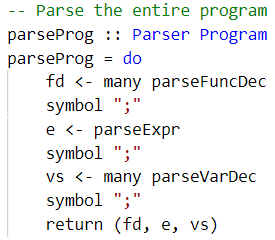
\includegraphics[scale=0.8]{img/code7}
		\end{columns}
	\end{itemize}

\begin{example}
	$f_1(x_1, x_2) = x_1, f_2(x_1) = x_1 + 2, f_3() = f_3() + 1; 3 + f_1(x_1 + 2, y); x_1 = 2, x_2 = 3, y = \underline{undef};$
\end{example}
\end{frame}

\begin{frame}{The Parser}
	\begin{columns}
		\column{0.5\textwidth}
		([(``$f_1$", [(Evar ``$x_1$"), (Evar ``$x_2$")], (Evar ``$x_1$")), (``$f_2$", [(Evar ``$x_1$")], (EOp (Evar ``$x_1$") PL (Enum (Just 2)))), (``$f_3$", [], (EOp (EFunc ``$f_3$" []) P (ENum 1)))],
		(EOp (ENum 3) P (EFunc ``$f_1$" [(EOp (EVar ``$x_1$") P (ENum 2)), (EVar ``y")])), [(``$x_1$", (Just 2)), (``$x_2$", (Just 3)), (``y", Nothing)])
		\column{0.5\textwidth}
		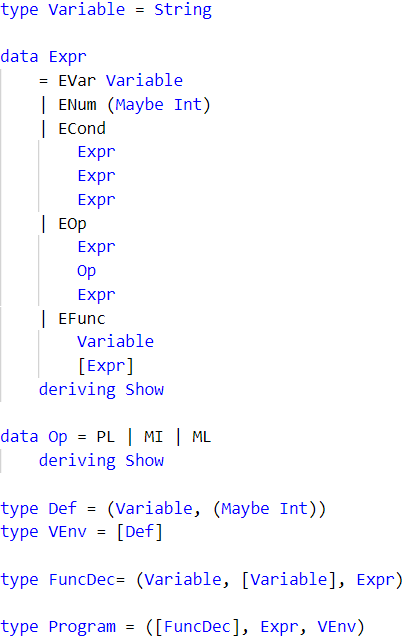
\includegraphics[scale=0.6]{img/code8}
	\end{columns}
\end{frame}

\section{Interpreter}
\begin{frame}{The Interpreter}
	\framesubtitle{Initially a simple translation job \dots}
	\begin{center}
		\begin{tikzpicture}
		\node (theory) {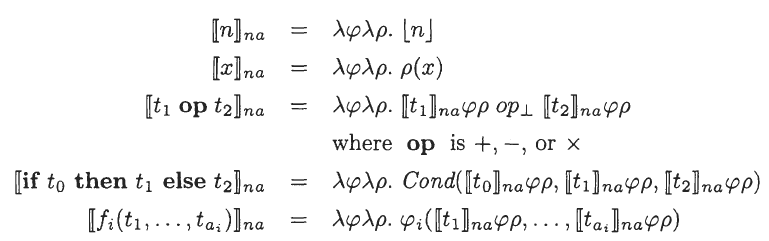
\includegraphics[scale=0.6]{img/rec2}};
		\node (code) [below=of theory] {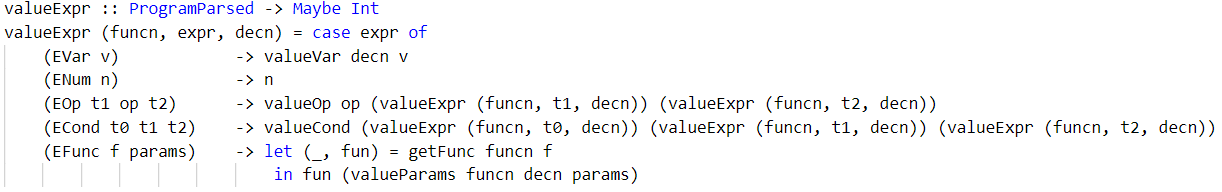
\includegraphics[width=\textwidth]{img/code2}};
		
		\draw [ultra thick,black,->] (theory) to (code);
		\end{tikzpicture}
	\end{center}
\end{frame}

\begin{frame}
	\frametitle{The Functional}
	\begin{center}
		\begin{tikzpicture}
		\node (theory) {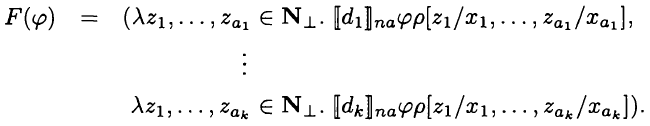
\includegraphics[scale=0.6]{img/rec3}};
		\node (code) [below=of theory] {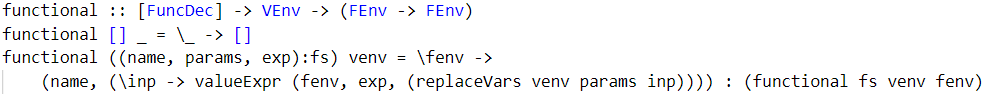
\includegraphics[width=\textwidth]{img/code3}};
		
		\draw [ultra thick,black,->] (theory) to (code);
		\end{tikzpicture}
	\end{center}
\end{frame}

\begin{frame}
	\frametitle{The Knaster-Tarski-Kleene theorem}
	\begin{center}
		\begin{tikzpicture}
		\node (theory) {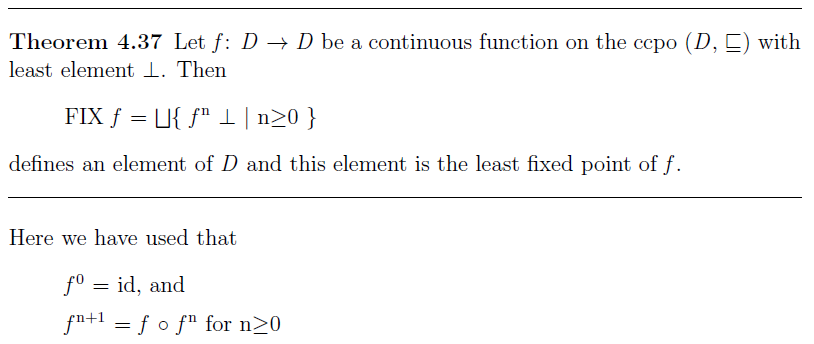
\includegraphics[scale=0.6]{img/fix5}};
		\node (code) [below=of theory] {
			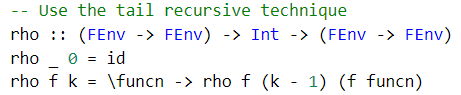
\includegraphics[scale=0.7]{img/code5}
			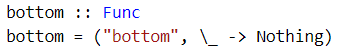
\includegraphics[scale=0.7]{img/code5.1}};
		
		\draw [ultra thick,black,->] (theory) to (code);
		\end{tikzpicture}
	\end{center}
\end{frame}

\begin{frame}
	\frametitle{The Tail Recursion}
	\begin{itemize}
		\item Definition of Functional function:
		\begin{align*}
		\texttt{factorial 0 r} &= \texttt{r}\\
		\texttt{factorial n r} &= \texttt{factorial (n - 1) (r * n)}
		\end{align*}
		\item Execution steps of an example:
		\begin{align*}
		\texttt{facAux 5 1} &= \texttt{factorial 4 5}\\
							&= \texttt{factorial 3 20}\\
							&= \texttt{factorial 2 60}\\
							&= \texttt{factorial 1 210}\\
							&= \texttt{factorial 0 120}\\
							&= 120
		\end{align*} 
	\end{itemize}
\end{frame}

\begin{frame}{The main functions}
	\begin{center}
		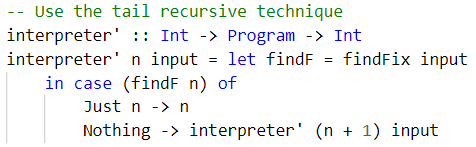
\includegraphics[scale=0.8]{img/code1}
		
	\end{center}
\vspace*{0.5cm}
\begin{center}
	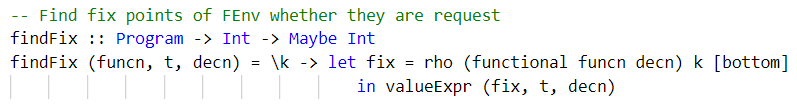
\includegraphics[width=\textwidth]{img/code4}
\end{center}
\end{frame}
\end{document}